\PassOptionsToPackage{unicode=true}{hyperref} % options for packages loaded elsewhere
\PassOptionsToPackage{hyphens}{url}
%
\documentclass[ignorenonframetext,aspectratio=169]{beamer}
\usepackage{pgfpages}
\setbeamertemplate{caption}[numbered]
\setbeamertemplate{caption label separator}{: }
\setbeamercolor{caption name}{fg=normal text.fg}
\beamertemplatenavigationsymbolsempty
% Prevent slide breaks in the middle of a paragraph:
\widowpenalties 1 10000
\raggedbottom
\setbeamertemplate{part page}{
\centering
\begin{beamercolorbox}[sep=16pt,center]{part title}
  \usebeamerfont{part title}\insertpart\par
\end{beamercolorbox}
}
\setbeamertemplate{section page}{
\centering
\begin{beamercolorbox}[sep=12pt,center]{part title}
  \usebeamerfont{section title}\insertsection\par
\end{beamercolorbox}
}
\setbeamertemplate{subsection page}{
\centering
\begin{beamercolorbox}[sep=8pt,center]{part title}
  \usebeamerfont{subsection title}\insertsubsection\par
\end{beamercolorbox}
}
\AtBeginPart{
  \frame{\partpage}
}
\AtBeginSection{
  \ifbibliography
  \else
    \frame{\sectionpage}
  \fi
}
\AtBeginSubsection{
  \frame{\subsectionpage}
}
\usepackage{lmodern}
\usepackage{amssymb,amsmath}
\usepackage{ifxetex,ifluatex}
\usepackage{fixltx2e} % provides \textsubscript
\ifnum 0\ifxetex 1\fi\ifluatex 1\fi=0 % if pdftex
  \usepackage[T1]{fontenc}
  \usepackage[utf8]{inputenc}
  \usepackage{textcomp} % provides euro and other symbols
\else % if luatex or xelatex
  \usepackage{unicode-math}
  \defaultfontfeatures{Ligatures=TeX,Scale=MatchLowercase}
\fi
\usetheme[]{Frankfurt}
\usecolortheme{beaver}
% use upquote if available, for straight quotes in verbatim environments
\IfFileExists{upquote.sty}{\usepackage{upquote}}{}
% use microtype if available
\IfFileExists{microtype.sty}{%
\usepackage[]{microtype}
\UseMicrotypeSet[protrusion]{basicmath} % disable protrusion for tt fonts
}{}
\IfFileExists{parskip.sty}{%
\usepackage{parskip}
}{% else
\setlength{\parindent}{0pt}
\setlength{\parskip}{6pt plus 2pt minus 1pt}
}
\usepackage{hyperref}
\hypersetup{
            pdftitle={Centers of diversity of crops and wild genetic diversity},
            pdfauthor={Deependra Dhakal},
            pdfborder={0 0 0},
            breaklinks=true}
\urlstyle{same}  % don't use monospace font for urls
\newif\ifbibliography
\setlength{\emergencystretch}{3em}  % prevent overfull lines
\providecommand{\tightlist}{%
  \setlength{\itemsep}{0pt}\setlength{\parskip}{0pt}}
\setcounter{secnumdepth}{0}

% set default figure placement to htbp
\makeatletter
\def\fps@figure{htbp}
\makeatother

\usepackage{booktabs}
\usepackage{longtable}
\usepackage{array}
\usepackage{multirow}
\usepackage{wrapfig}
\usepackage{float}
\usepackage{colortbl}
\usepackage{pdflscape}
\usepackage{tabu}
\usepackage{threeparttable}
\usepackage{threeparttablex}
\usepackage[normalem]{ulem}
\usepackage{makecell}
\usepackage{xcolor}
\usepackage{tikz} % required for image opacity change
\usepackage[absolute,overlay]{textpos} % for text formatting

% this font option is amenable for beamer
\setbeamerfont{caption}{size=\tiny}

\title{Centers of diversity of crops and wild genetic diversity}
\author{Deependra Dhakal}
\providecommand{\institute}[1]{}
\institute{GAASC, Baitadi \and Tribhuwan University}
\date{Academic year 2019-2020}

\begin{document}
\frame{\titlepage}

\begin{frame}
\tableofcontents[hideallsubsections]
\end{frame}
\begin{frame}

\begin{figure}

{\centering 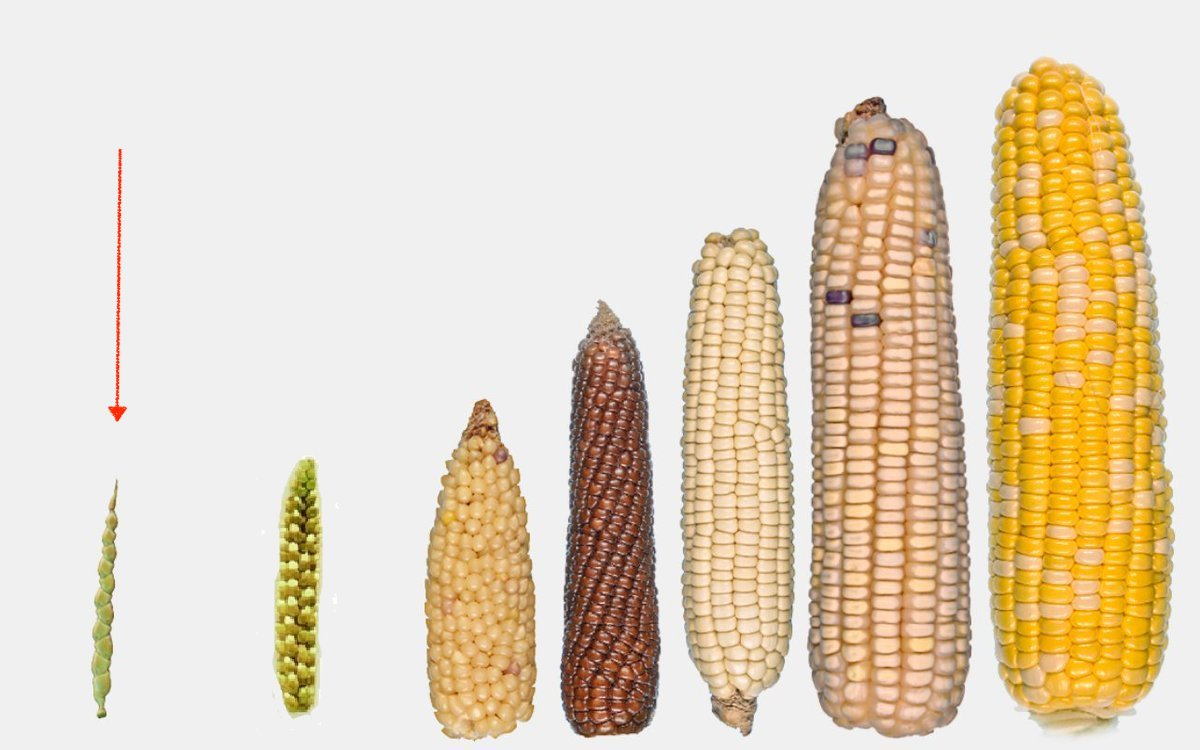
\includegraphics[width=0.55\linewidth]{./../images/maize_breeding} 

}

\caption{Evolutionary history of maize}\label{fig:maize-domestication}
\end{figure}

\end{frame}

\hypertarget{domestication}{%
\section{Domestication}\label{domestication}}

\hypertarget{what-is-a-weed}{%
\subsection{What is a weed?}\label{what-is-a-weed}}

\begin{frame}{Weed}
\protect\hypertarget{weed}{}

\begin{itemize}
\tightlist
\item
  ``A plant in the wrong place''
\item
  How accurate is the definition ?
\item
  We define weeds as plants we do not want that compete for resources
  with those we do want.
\item
  Clearly we have criteria about which plants we want and those that
  fail those criteria.
\item
  In evolutionary terms, it is the cultivated plants that are ``fitter''
  than the weeds, as they have characteristics which we want, and since
  in the fi eld and the garden we have largely substituted ourselves for
  nature, and here it is us who control the evolutionary process.
\item
  However, many commercially grown plants survive as volunteer weeds, or
  ``escapes'', in either the same, or different, regions to those in
  which they are most commonly grown commercially.
\end{itemize}

\end{frame}

\begin{frame}{}
\protect\hypertarget{section}{}

\begin{block}{}
The gap between the wild and the cultivated is all about the difference between nature's requirements and ours.
\end{block}

(Kingsbury 2009)

\end{frame}

\begin{frame}{}
\protect\hypertarget{section-1}{}

\begin{figure}

{\centering 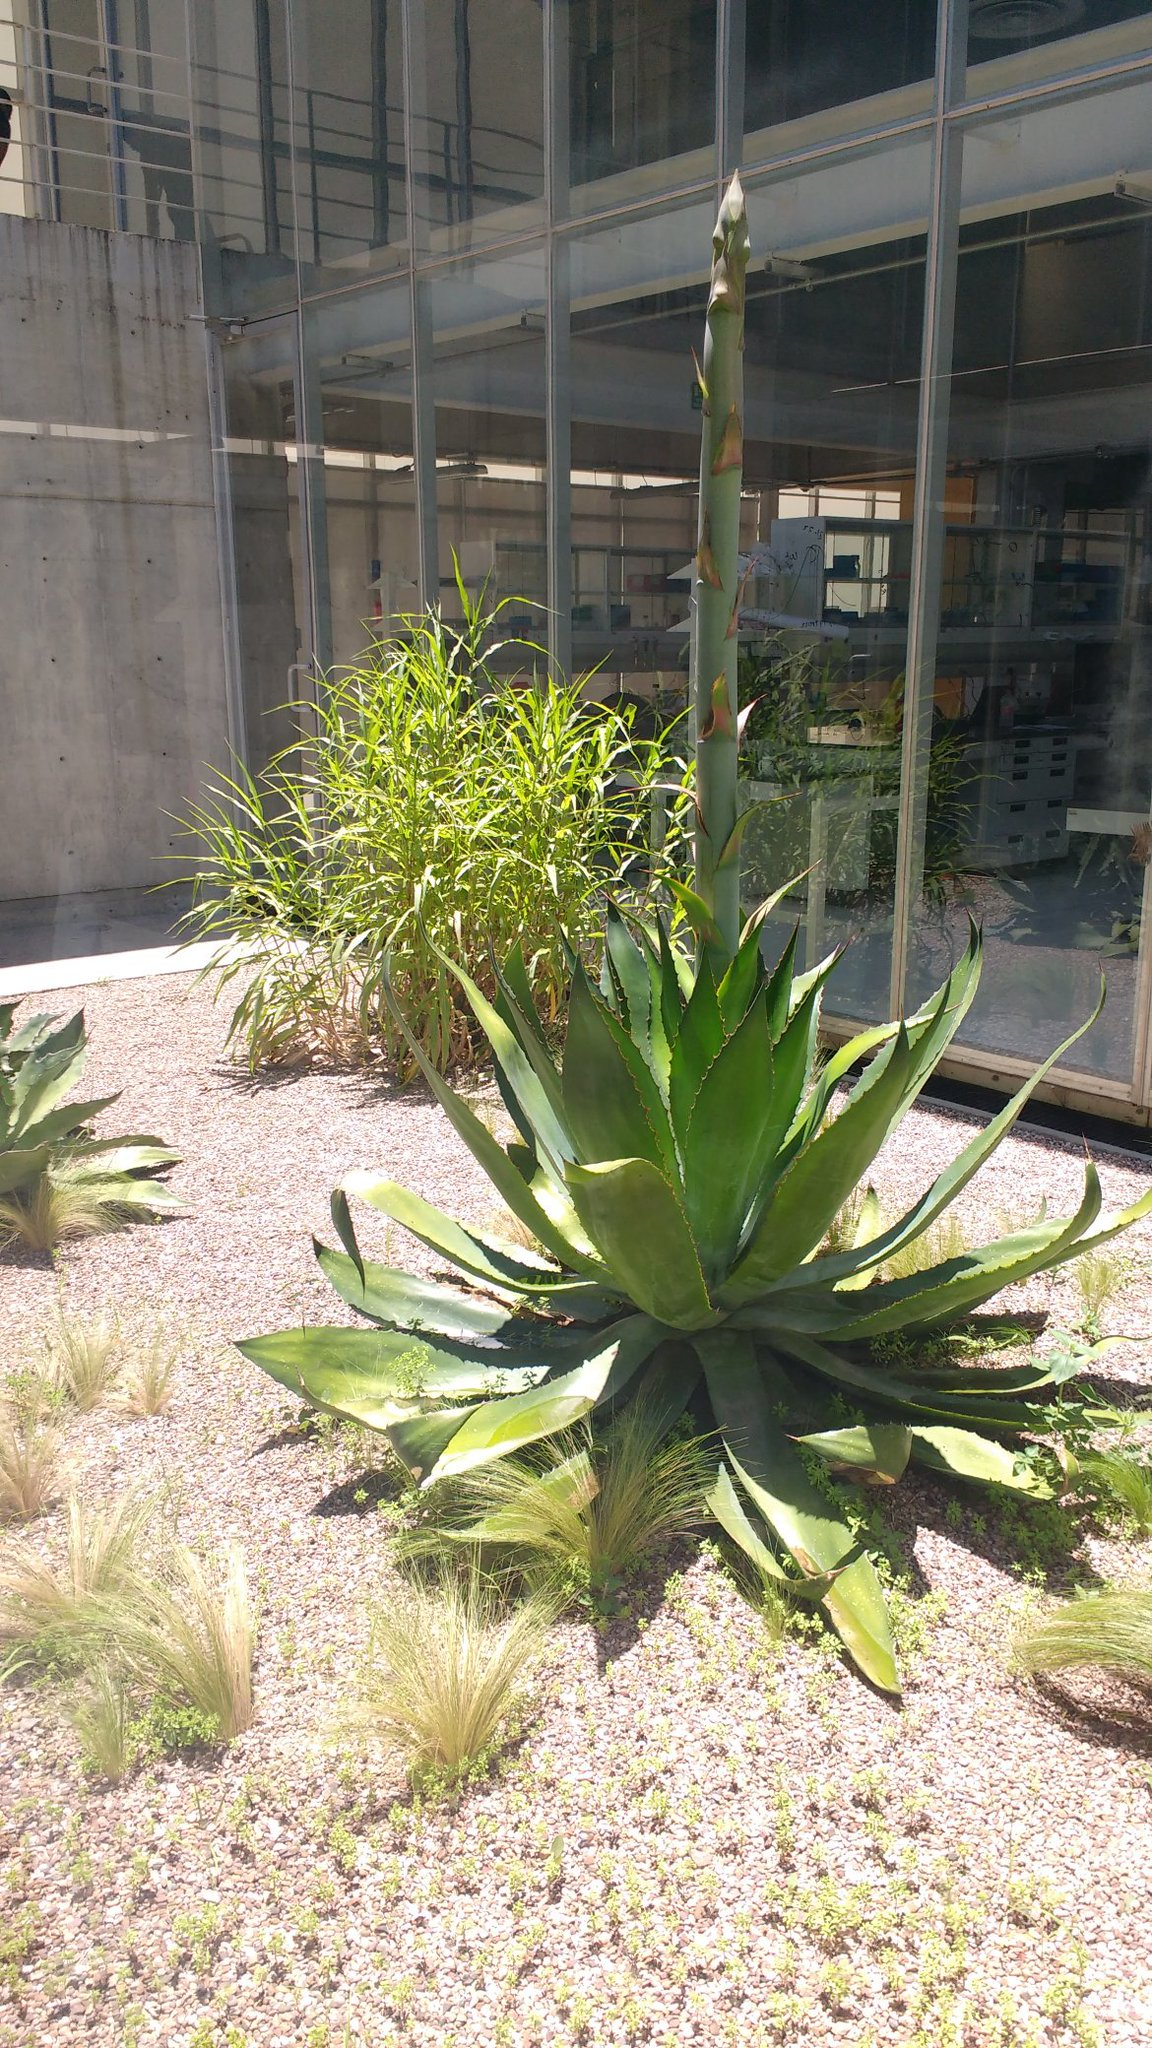
\includegraphics[width=0.26\linewidth]{./../images/Perennial_teosinte} 

}

\caption{Perennial teosinte}\label{fig:weed-vs-crop}
\end{figure}

\end{frame}

\begin{frame}{Definition}
\protect\hypertarget{definition}{}

\begin{block}{}
a plant population has been domesticated when it has been substantially altered from the wild state and certainly when it has been so altered to be unable to survive in the wild
\end{block}

N.W. Simmonds

\begin{itemize}
\tightlist
\item
  Domestication is the process by which genetic changes (shifts) in wild
  plants are brought about through a selection process imposed by
  humans.
\end{itemize}

\end{frame}

\begin{frame}{}
\protect\hypertarget{section-2}{}

\begin{itemize}
\tightlist
\item
  Because of the roles of humans, the process results characteristics
  that are beneficial to humans but some that would be disadvantageous
  for plants in their natural habitats.
\item
  Results are the plants that are adapted to supervised cultural
  conditions and which posses characteristics that are preferred by
  producers and consumers.
\item
  E.g. Modern corn stripped is completely of its seed dispersal ability.
\item
  \emph{Domesticators}
\item
  Both wild and domesticated populations are subject to evolution
\item
  Forces of selection determine what will be domesticated and that which
  will continue in wild

  \begin{itemize}
  \tightlist
  \item
    The natural selection favours plant phenotypes which have the
    greatest chance of survival, reproduction, and distribution of
    progeny.
  \item
    Human selection is the result of conscious decisions by a farmer or
    plant breeder to keep the progeny of a particular parent and discard
    others.
  \end{itemize}
\end{itemize}

\end{frame}

\hypertarget{domestication-syndrome-changes-in-plant-species-under-domestication}{%
\subsection{Domestication syndrome (Changes in plant species under
domestication)}\label{domestication-syndrome-changes-in-plant-species-under-domestication}}

\begin{frame}{}
\protect\hypertarget{section-3}{}

\begin{table}[t]

\caption{\label{tab:domestication-syndrome}Changes in plants under domestication}
\centering
\fontsize{6}{8}\selectfont
\begin{tabular}{>{\raggedright\arraybackslash}p{16em}>{\raggedright\arraybackslash}p{40em}}
\toprule
General effect & Specific traits altered\\
\midrule
\rowcolor{gray!6}  Increased seedling vigor (more plants germinating) & Loss of seed or tuber dormancy\\
 & Large seeds\\
\rowcolor{gray!6}  Modified reproductive system & Increased selfing\\
 & Reduced complexity of reproductive organs\\
\rowcolor{gray!6}   & Vegetatively reproducing plants\\
\addlinespace
 & Altered photoperiod sensitivity\\
\rowcolor{gray!6}   & Shift in sex form of species\\
 & Promotion of asexual reproduction\\
\rowcolor{gray!6}  Increased number of seeds harvested & Non-shattering\\
 & Reduced number of branches (more fruits per branch)\\
\bottomrule
\end{tabular}
\end{table}

\end{frame}

\begin{frame}{}
\protect\hypertarget{section-4}{}

\begin{table}[t]

\caption{\label{tab:domestication-syndrome2}Changes in plants under domestication (...continued)}
\centering
\fontsize{6}{8}\selectfont
\begin{tabular}{>{\raggedright\arraybackslash}p{16em}>{\raggedright\arraybackslash}p{40em}}
\toprule
General effect & Specific traits altered\\
\midrule
\rowcolor{gray!6}  Increased appeal to consumers & Attractive fruit/seed colors and patterns\\
 & Enhanced flavor, texture, and taste of seeds/fruits/tubers (food parts)\\
\rowcolor{gray!6}   & Reduced toxic principles (safer food)\\
 & Larger fruits\\
\rowcolor{gray!6}   & Reduces spikiness\\
\addlinespace
 & Increase in economic yield (HI)\\
\rowcolor{gray!6}  Altered plant architecture and growth habit & Compact growth habit (Determinacy, reduced plant size, dwarfism)\\
 & Reduced branching\\
\rowcolor{gray!6}   & Decreases in variability within a variety\\
Change in developmental phenology & Change in life cycle (normally from perennial to annual for seed crops, and from annual to biennial for vegetable crops)\\
\bottomrule
\end{tabular}
\end{table}

\end{frame}

\begin{frame}{Wild versus domestication traits}
\protect\hypertarget{wild-versus-domestication-traits}{}

\begin{columns}[T,onlytextwidth]
  
  \column{0.5\textwidth}
  
\begin{figure}
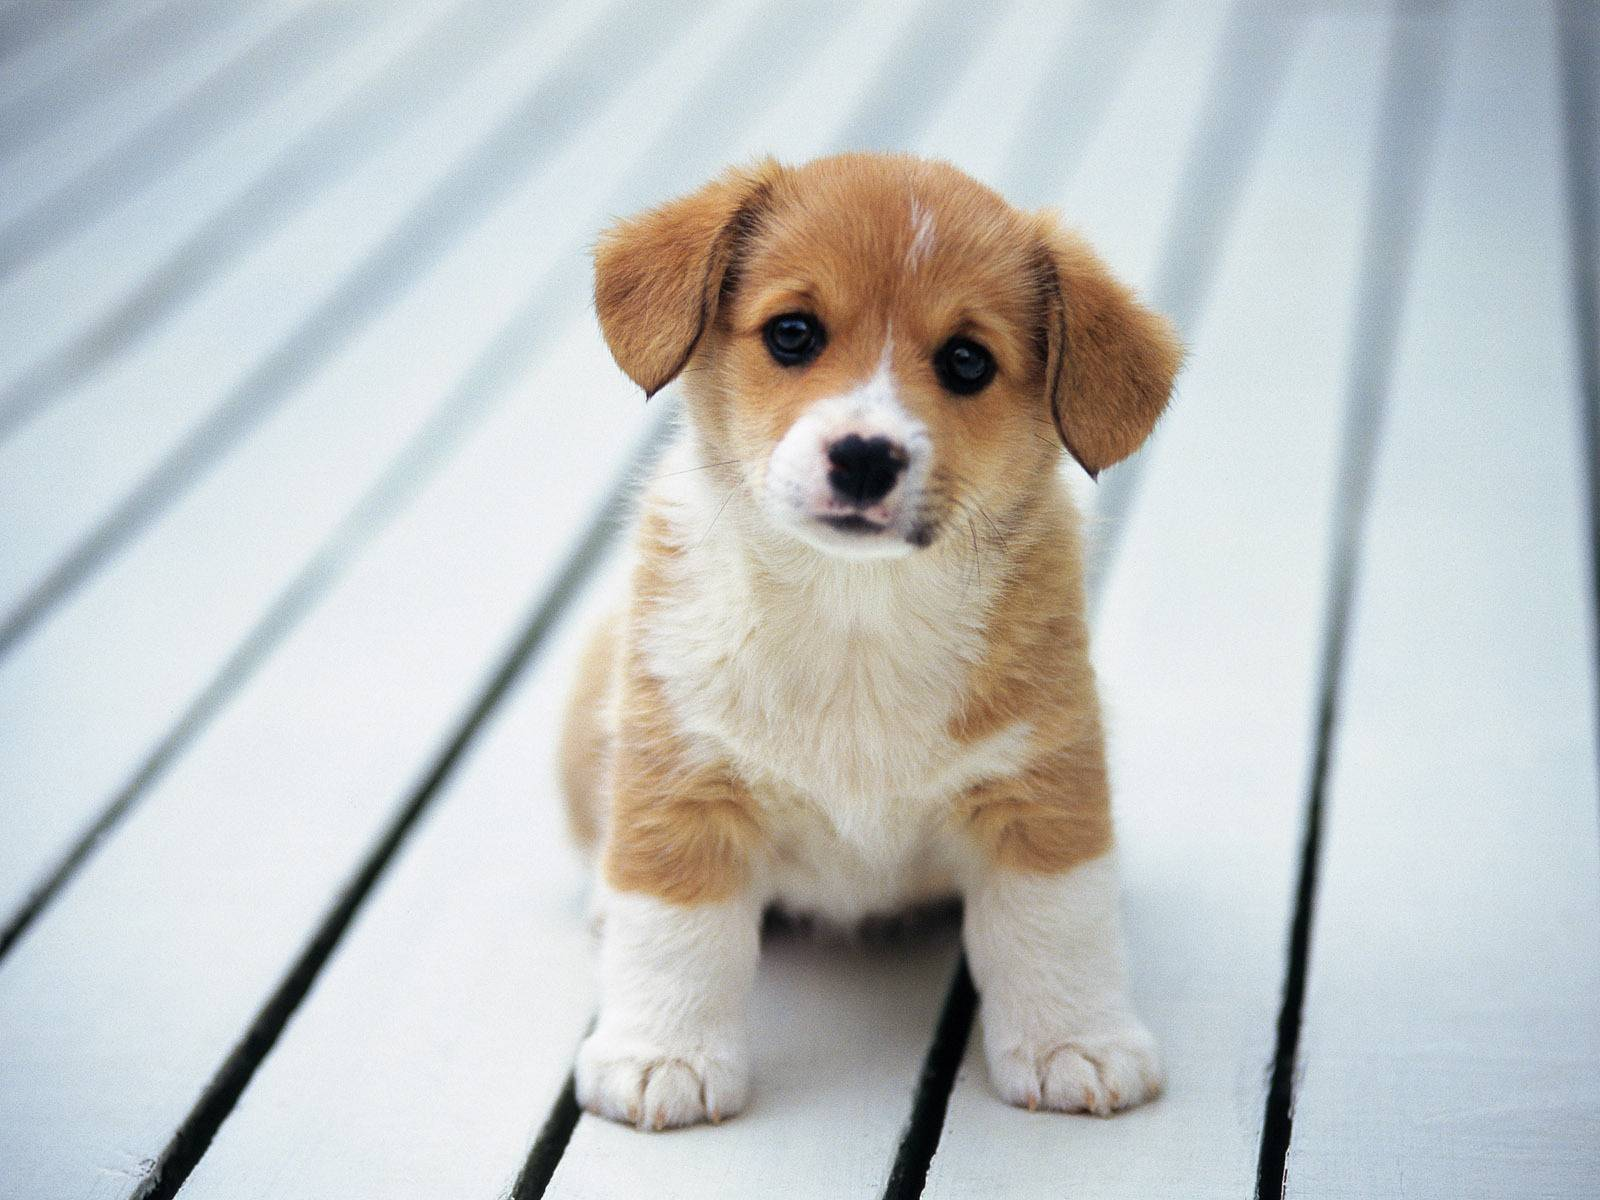
\includegraphics[width=0.8\linewidth]{./../images/domestic_dog_puppy} \caption{Domesticated dog}\label{fig:domesticated}
\end{figure}

  \column{0.5\textwidth}

\begin{figure}
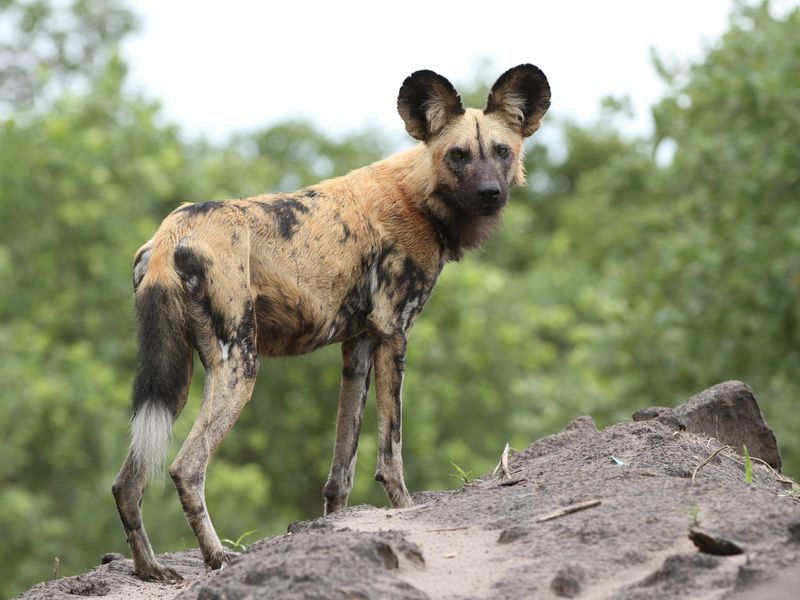
\includegraphics[width=0.8\linewidth]{./../images/wild_dog_african} \caption{Wild dog}\label{fig:wild}
\end{figure}

\end{columns}

\end{frame}

\begin{frame}{Wild verus domestication traits (context)}
\protect\hypertarget{wild-verus-domestication-traits-context}{}

\begin{itemize}
\item
  Wild cereal plants tend to have many small seeds at maturity and
  disperse their seed by shattering. These seeds also are likely to be
  attached to a strong awn to aid dispersal.
\item
  Similarly, wild potato species produce many small tubers, have their
  tubers develop at the end of very long stolons (so that daughter
  plants do not have to occupy ground too close to the parent), and many
  have tubers with high levels of toxin, which discourage animals from
  eating them.
\item
  Breeders have developed cereal cultivars which have fewer, but larger
  seeds, that do not shatter their seeds at maturity and that have a
  non-persistent awn.
\end{itemize}

\end{frame}

\begin{frame}{}
\protect\hypertarget{section-5}{}

\begin{itemize}
\item
  Similarly potato breeders have selected plants with fewer, but larger
  tubers, shorter stolons and with reduced levels of toxins in the
  tuber.
\item
  Human selection also has produced crops that are more uniform in the
  expression of many of their characteristics. For example, they have
  selected seeds that all mature at the same time, with uniform
  germination, and fruits with uniform fruit size and shape.
\item
  In more recent times plant breeders' selection has tended to result in
  shorter plants, greater harvest index, and increased ease of harvest
  (especially mechanized).
\end{itemize}

\end{frame}

\begin{frame}{}
\protect\hypertarget{section-6}{}

\begin{figure}

{\centering 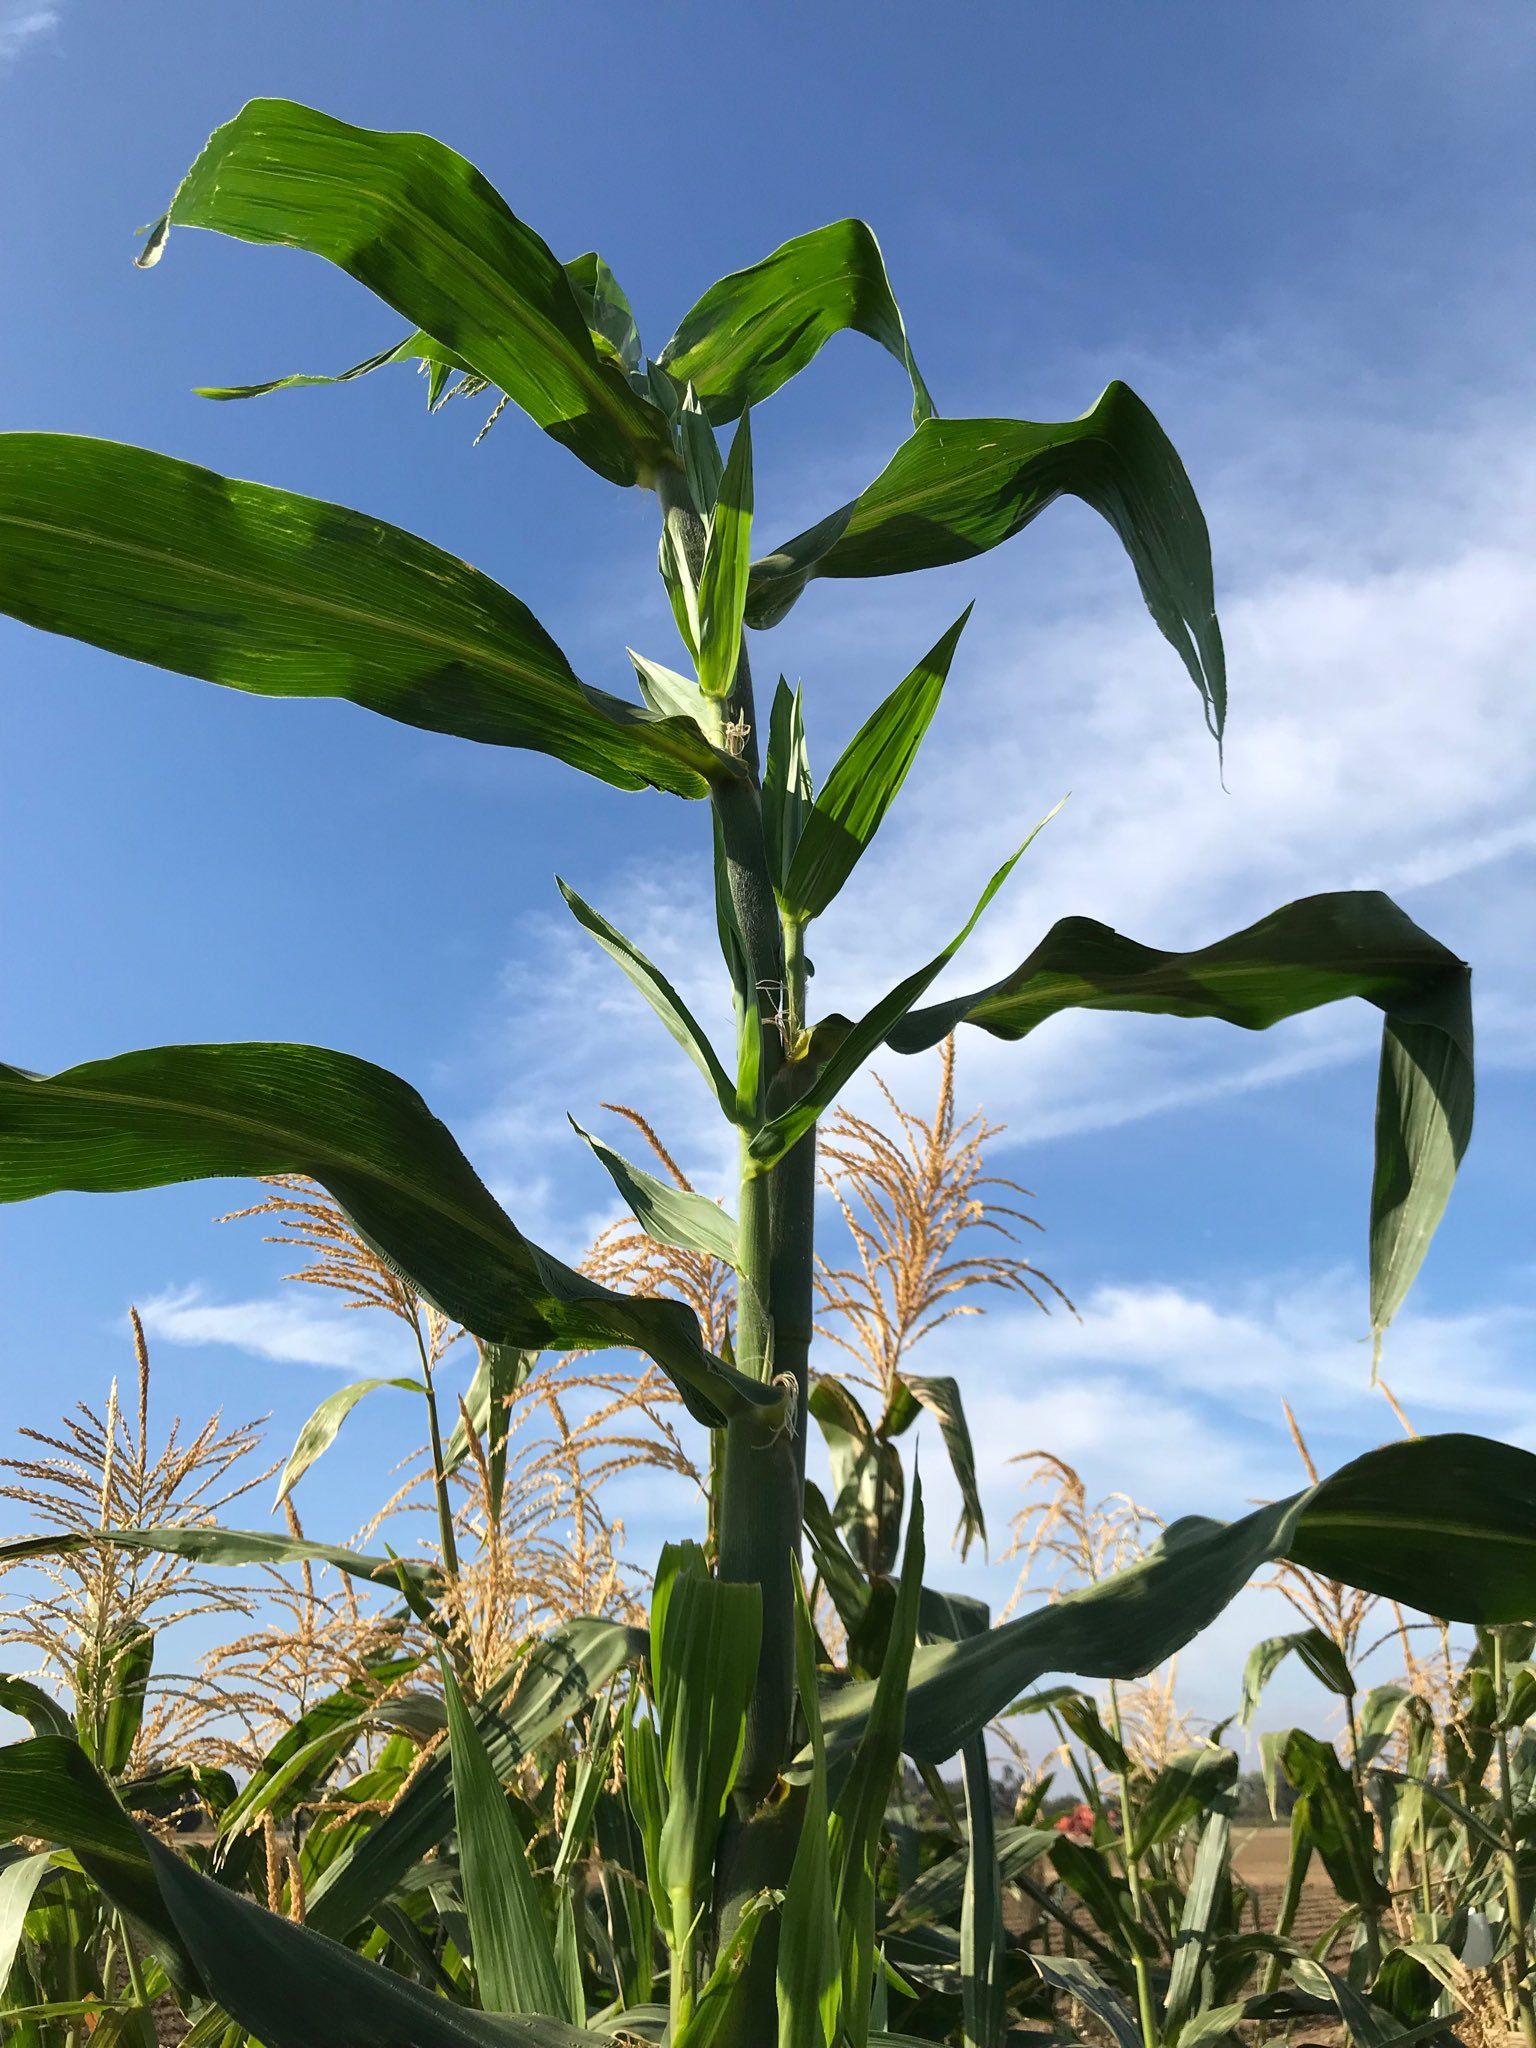
\includegraphics[width=0.4\linewidth]{./../images/Teosinte_maize_hybrid_cross} 

}

\caption{Teosinte maize hybrid}\label{fig:unnamed-chunk-1}
\end{figure}

\end{frame}

\begin{frame}{When did domestication appear?}
\protect\hypertarget{when-did-domestication-appear}{}

In the Euphrates valley of northern Syria, reliable signs of
morphological domestication, indicated by the partial loss of the
dispersal mechanism in emmer and barley, are found in the earliest
levels at the sites of Halula and Abu Hureyra 2, dated to c. 10,000 BP
These are full-scale farming sites, which have domestic animals and
cover a surface area at least ten times larger than the PPNA sites.
Elsewhere the same tell-tale abscission scars left on spikelet bases
were found at the sites of Nevali Cori, Cayonu and Cafer Hoyuk dated to
c. 10,500 years ago. The later date for domestication on the Euphrates
in northern Syria may be due to a gap in the archaeological record. At
these early domestication sites, wild types persist alongside the
domestic types (van Zeist and de Roller 1994, de Moulins 1997, Pasternak
1998, Tanno and Willcox 2006).

\end{frame}

\begin{frame}{Germplasm}
\protect\hypertarget{germplasm}{}

\begin{itemize}
\tightlist
\item
  Germplasm refers to the genetic material that can be used to
  perpetuate a species or population
\item
  Germplasm provides the material used to initiate a breeding program
\item
  Sometimes only germplasm screening and evaluation is practiced for
  introduction of improved variety in a region
\item
  Certain institutional sets-ups such as gene banks are charged with the
  responsibility of assembling, cataloguing, storing and managing large
  number of germplasm. This allows for quick retrieval.
\end{itemize}

\end{frame}

\hypertarget{gene-pool}{%
\subsection{Gene pool}\label{gene-pool}}

\begin{frame}{Background}
\protect\hypertarget{background}{}

J.R. Harlan and J.M.J. de Wet proposed a categorization of gene pools of
cultivated crops according to the feasibility of gene transfer or gene
flow from those species to the crop species.

\begin{figure}
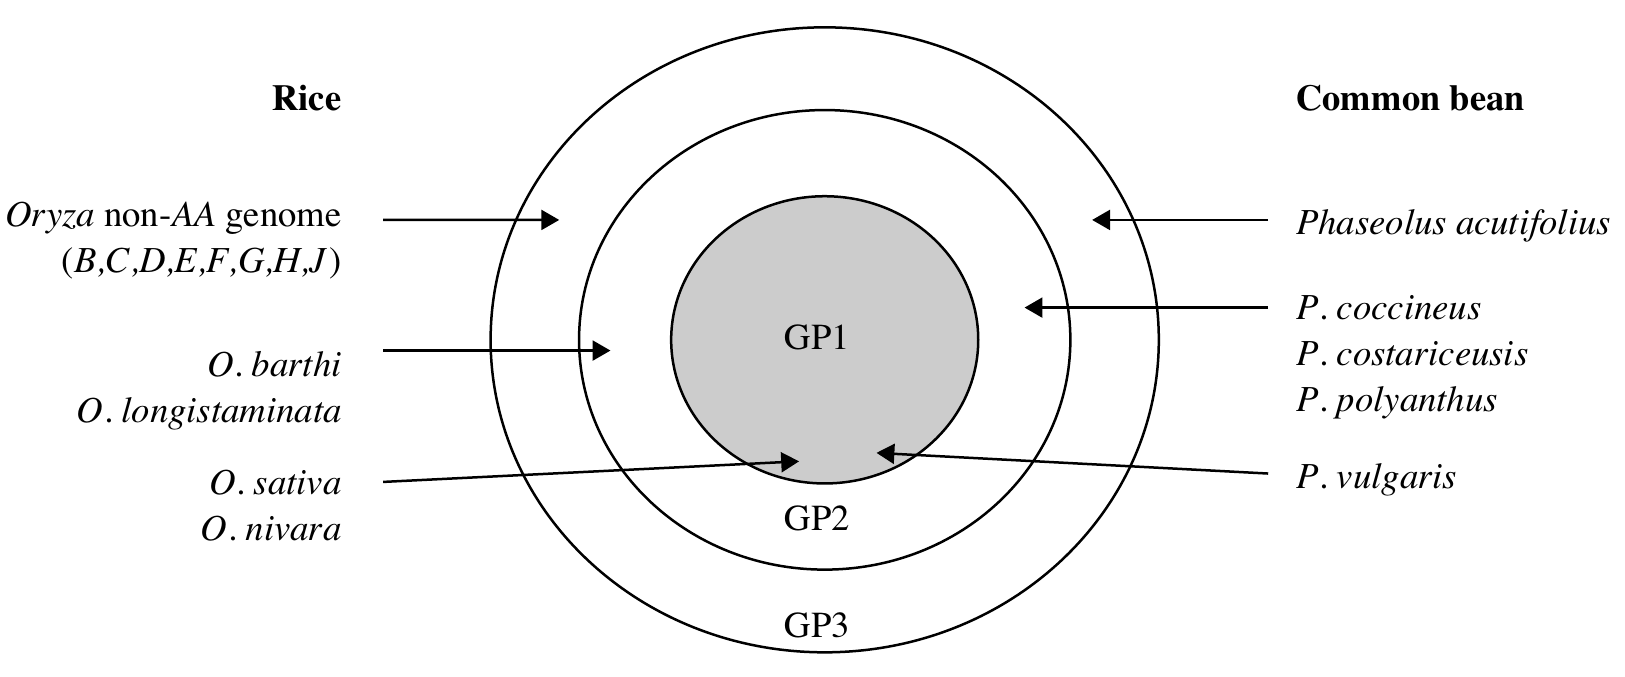
\includegraphics[width=0.45\linewidth]{./../images/crop_gene_pools} \caption{Crop gene pools; A system proposed by Harlan}\label{fig:gene-pools}
\end{figure}

\end{frame}

\begin{frame}{Types of gene pool}
\protect\hypertarget{types-of-gene-pool}{}

\begin{itemize}
\tightlist
\item
  \emph{Primary gene pool (GP1)}

  \begin{itemize}
  \tightlist
  \item
    GP1 consists of biological species that can be intercrossed easily
    (interfertile) without any problems with fertility of the progeny.
    That is, there is no restriction to gene exchange between members of
    the group. This group may contain both cultivated and wild
    progenitors of the species.
  \end{itemize}
\item
  \emph{Secondary gene pool (GP2)}

  \begin{itemize}
  \tightlist
  \item
    Members of this gene pool include both cultivated and wild relatives
    of the crop species. They are more distantly related and have
    crossability problems. Nonetheless, crossing produces hybrids and
    derivatives that are sufficiently fertile to allow gene flow. GP2
    species can cross with those in GP1, with some fertility of the F1,
    but more difficulty with success.
  \end{itemize}
\item
  \emph{Tertiary gene pool (GP3)}

  \begin{itemize}
  \tightlist
  \item
    GP3 involves the outer limits of potential genetic resources. Gene
    transfer by hybridization between GP1 and GP3 is very problematic,
    resulting in lethality, sterility, and other abnormalities. To
    exploit germplasm from distant relatives, tools such as embryo
    rescue and bridge crossing may be used to nurture an embryo from a
    wide cross to a full plant and to obtain fertile plants.
  \end{itemize}
\end{itemize}

\end{frame}

\hypertarget{origin-and-diversity}{%
\section{Origin and diversity}\label{origin-and-diversity}}

\hypertarget{the-vavilov-concept}{%
\subsection{The Vavilov Concept}\label{the-vavilov-concept}}

\begin{frame}{}
\protect\hypertarget{section-7}{}

\begin{itemize}
\item
  Nikolai I. Vavilov (1887-1942), the Russian botanist and plant
  breeder, demonstrated the existence of `centres of origin' of
  cultivated plants (more correctly named today as `centres of
  diversity'), in which can be found the highest level of genetic
  variability of a species. This variability, which arises in nature by
  mutation spontaneous hybridization, introgression and changes in
  chromosome form and number, provides the means by which adaptation to
  heterogenous environments can occur.
\item
  It allows the breeder to identify sources of variation for specific
  characteristics. The extension of this principle to related species
  was formulated by Vavilov in his `law of homologous series of
  variation'. This law allows the prediction of the appearance of a
  given type of mutation in a plant species when such a type has been
  found in another species phylogenetically related to the first.
\item
  Defined plant breeding as `plant evolution directed by man'; concept
  of `applied plant genetics'.
\end{itemize}

\end{frame}

\hypertarget{domestication-and-origin-of-major-crop-species}{%
\subsection{Domestication and origin of major crop
species}\label{domestication-and-origin-of-major-crop-species}}

\begin{frame}{}
\protect\hypertarget{section-8}{}

\begin{table}[t]

\caption{\label{tab:domestication-origin}Estimated time of domestication and centre of origin of major crop species; @brown2014plant, Page 23}
\centering
\fontsize{6}{8}\selectfont
\begin{tabular}{>{\raggedright\arraybackslash}p{8em}>{\raggedright\arraybackslash}p{12em}>{\raggedright\arraybackslash}p{8em}>{\raggedright\arraybackslash}p{12em}}
\toprule
Crop category & Crop & Length of time domesticated (years) & Possible region of origin\\
\midrule
\rowcolor{gray!6}  Cereals & Maize, Zea mays & 7000 & Mexico, Central America\\
Cereals & Rice, Oryza sativa & 4500 & Thailand, Southern China\\
\rowcolor{gray!6}  Cereals & Wheat, Triticum spp. & 8500 & Syria, Jordan, Israel, Iraq\\
Cereals & Barley, Hordeum vulgare & 9000 & Syria, Jordan, Israel, Iraq\\
\rowcolor{gray!6}  Cereals & Sorghum, Sorghum bicolor & 8000 & Equatorial Africa\\
\addlinespace
Oilseeds & Soybean, Glycine max & 2000 & North China\\
\rowcolor{gray!6}  Oilseeds & Oil palm, Elaeis guineensis & 9000 & Central Africa\\
Oilseeds & Coconut palm, Cocos nucifera & 100 & Southern Asia\\
\rowcolor{gray!6}  Oilseeds & Rapeseed, Brassica napus & 500 & Mediterranean Europe\\
Oilseeds & Sunflower, Helianthus annus & 3000 & Western United States\\
\addlinespace
\rowcolor{gray!6}  Pulses & Beans, Phaseolus spp & 7000 & Centra America, Mexico\\
Pulses & Lentil, Lens culinaris & 7000 & Syria, Jordan, Israel, Iraq\\
\rowcolor{gray!6}  Pulses & Peas, Pisum sativum & 9000 & Syria, Jordan, Israel, Iraq\\
Root crops & Potato, Solanum tuberosum & 7000 & Peru\\
\rowcolor{gray!6}  Root crops & Cassava, Manihot esculenta & 5000 & Brazil, Mexico\\
\bottomrule
\end{tabular}
\end{table}

\end{frame}

\begin{frame}{}
\protect\hypertarget{section-9}{}

\begin{table}[t]

\caption{\label{tab:domestication-origin2}Estimated time of domestication and centre of origin of major crop species; @brown2014plant, Page 23 (...continued)}
\centering
\fontsize{6}{8}\selectfont
\begin{tabular}{>{\raggedright\arraybackslash}p{8em}>{\raggedright\arraybackslash}p{12em}>{\raggedright\arraybackslash}p{8em}>{\raggedright\arraybackslash}p{12em}}
\toprule
Crop category & Crop & Length of time domesticated (years) & Possible region of origin\\
\midrule
\rowcolor{gray!6}  Root crops & Sweet potato, Ipomoea batatas & 6000 & South Central America\\
Root crops & Sugar beet, Beta vulgaris & 300 & Mediterranean Europe\\
\rowcolor{gray!6}  Vegetables & Tomato, Lycopersicum esculentum & 3000 & Western South America\\
Vegetables & Cabbage, Brassica oleracea & 3000 & Mediterranean Europe\\
\rowcolor{gray!6}  Vegetables & Onion, Allium spp. & 4500 & Iran, Afganistan, Pakistan\\
\addlinespace
Fruit & Orange, Citrus sinensis & 9000 & South-east Asia\\
\rowcolor{gray!6}  Fruit & Apple, Malus spp. & 3000 & Asia Minor, Central Asia\\
Fruit & Grape, Vitis spp. & 7000 & Eastern Asia\\
\rowcolor{gray!6}  Fruit & Banana, Musa acuminata, M. balbisiana & 4500 & South-east Asia\\
Others & Cotton, Gossypium spp. & 4500 & Centra America, Brazil\\
\addlinespace
\rowcolor{gray!6}  Others & Coffee, Coffea spp. & 500 & West Ethiopia\\
Others & Rubber, Hevea brasiliensis & 200 & Brazil, Bolivia, Paraguay\\
\rowcolor{gray!6}  Others & Alfalfa, Medicago sativa & 4000 & Iran, Northern Pakistan\\
\bottomrule
\end{tabular}
\end{table}

\end{frame}

\begin{frame}{Rice}
\protect\hypertarget{rice}{}

\begin{itemize}
\tightlist
\item
  Probably originated 130 MYA (Virmani and IIyas-Ahmed, 2007)
\item
  Spread as wild grass in Gondwanaland.
\item
  Both cultivated species -- \emph{O. sativa} and \emph{O. glaberrima}
  (tropical West african rice) originated from common ancestor.
\item
  Wild progenitor of \emph{O. sativa} is common asian wild rice called
  \emph{O. rufipogon} (has perennial to annual types).
\item
  Annual types of the wild progenitor called \emph{O. nivara} resulted
  in present day asian rice.
\item
  Alternative hypotheses: two distinct subspecies of rice (
  \emph{indica} and \emph{japonica}) arose from different wild variants
  of \emph{O. rufipogon}.
\end{itemize}

\end{frame}

\begin{frame}{Rice (\ldots{}continued)}
\protect\hypertarget{rice-continued}{}

\begin{figure}
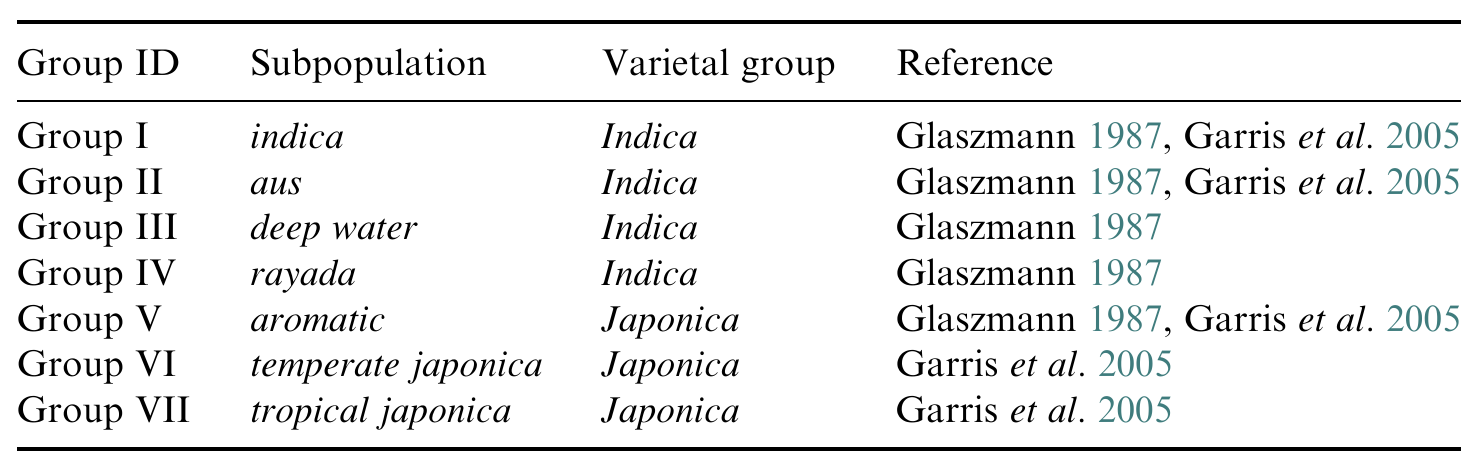
\includegraphics[width=0.45\linewidth]{./../images/rice_subpopulations} \caption{The recognized subpopulations of \textit{Oryza sativa}}\label{fig:subpopulations-rice}
\end{figure}

\end{frame}

\begin{frame}{Rice (\ldots{}continued)}
\protect\hypertarget{rice-continued-1}{}

\begin{itemize}
\tightlist
\item
  First archaeological evidence of rice cultivation leads to Yangtze
  valley of eastern China.
\item
  Domestication has resulted in alterations to a large array of
  morphological traits:

  \begin{itemize}
  \tightlist
  \item
    Seed shattering behavior
  \item
    Grain coloration
  \item
    Grain size enlargement
  \item
    Prostrate to erect growth habit
  \item
    Reduced seed dormancy
  \end{itemize}
\item
  Genetic factors contributing to domestication syndrome
  \emph{Shattering4 (Sha4)} on chromosome 4 and black hull by
  \emph{Black hull (Bh4)} on chromosome 4.
\end{itemize}

\end{frame}

\begin{frame}{Maize}
\protect\hypertarget{maize}{}

\begin{itemize}
\tightlist
\item
  Domestication history based on 7100 year old maize pollen from San
  Andres.
\item
  Initially cultivated in seasonal tropical forest of southwestern
  mexico.
\item
  Originated from annual teosinte (\emph{Zea mays} subspecies
  \emph{parviglumis}) around 9000 years ago in mid to lowland regions.
\item
  Later on admixture occured among \emph{parviglumis} and
  \emph{mexicana} (highland type) subspecies.
\end{itemize}

\end{frame}

\begin{frame}{Wheat}
\protect\hypertarget{wheat}{}

\begin{figure}
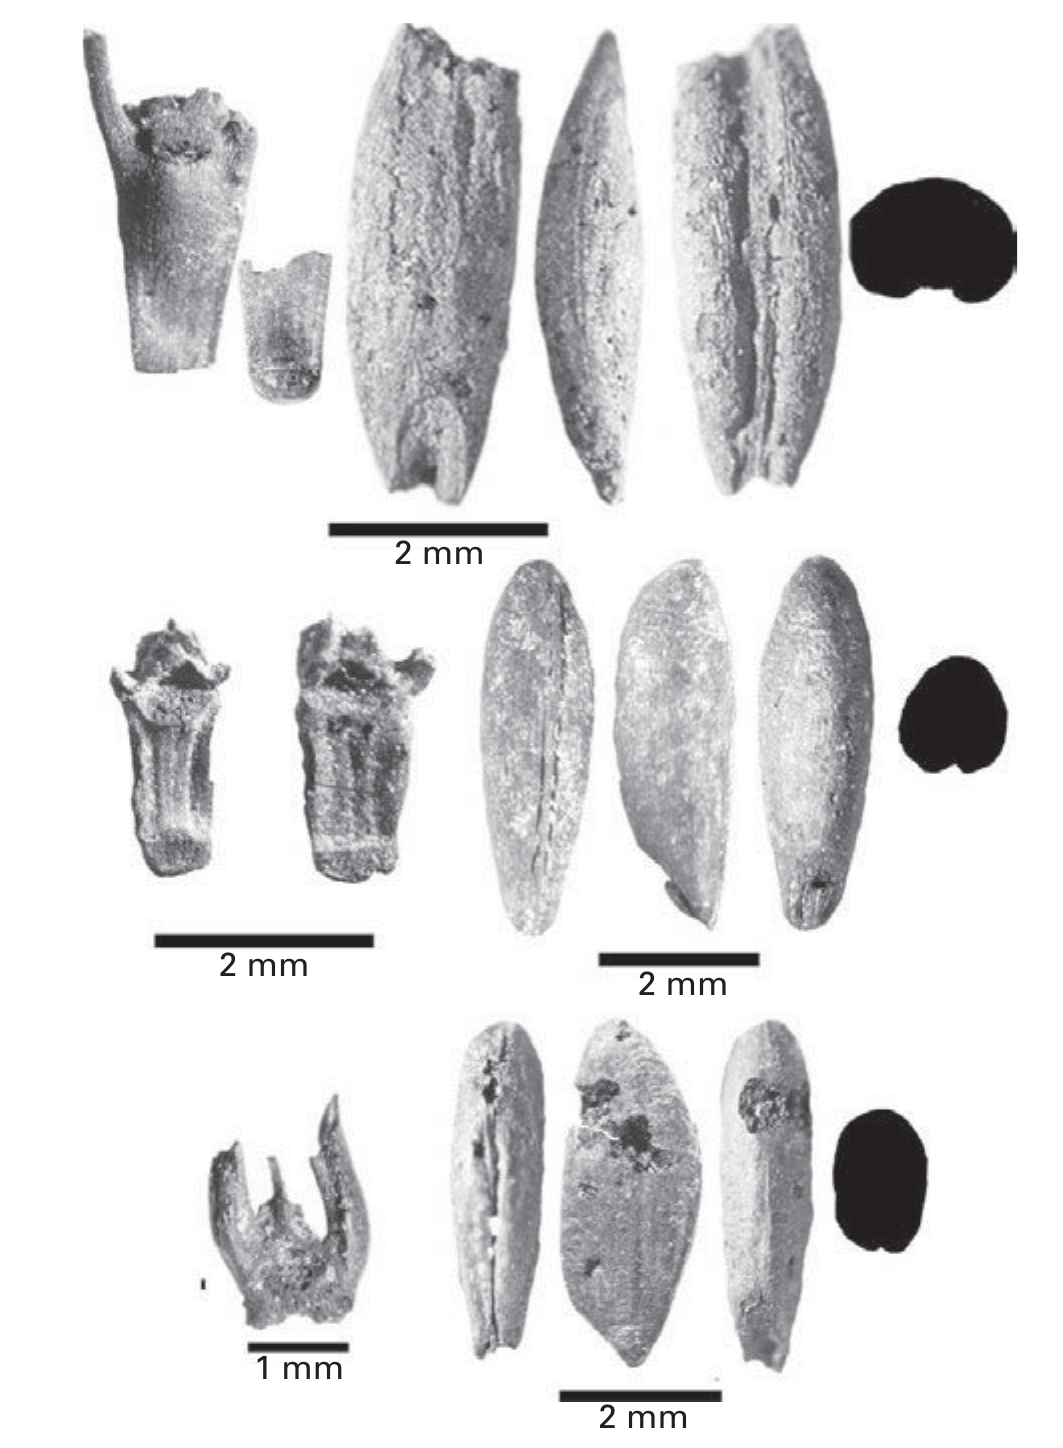
\includegraphics[width=0.3\linewidth]{./../images/charred_grass_grains} \caption{Charred wild cereal spikelet bases (left) and grains (right). Top, Hordeum spontaneum (wild barley) from Jerf el Ahmar. Middle, Secale sp. (rye) from Jerf el Ahmar. Bottom, Triticum boeoticum (single-grain einkorn) from Tell Qaramel. Note the basal abscission scar seen in the barley (top row, second from the left) and for rye the lower end of the rye spikelet bases (second row, first and second from left) is more reliable than the upper scar for distinguishing between wild and domestic.}\label{fig:wheat-barley-archaeology}
\end{figure}

\end{frame}

\hypertarget{megacentres-of-cutivated-plants}{%
\subsection{Megacentres of cutivated
plants}\label{megacentres-of-cutivated-plants}}

\begin{frame}{}
\protect\hypertarget{section-10}{}

\begin{figure}
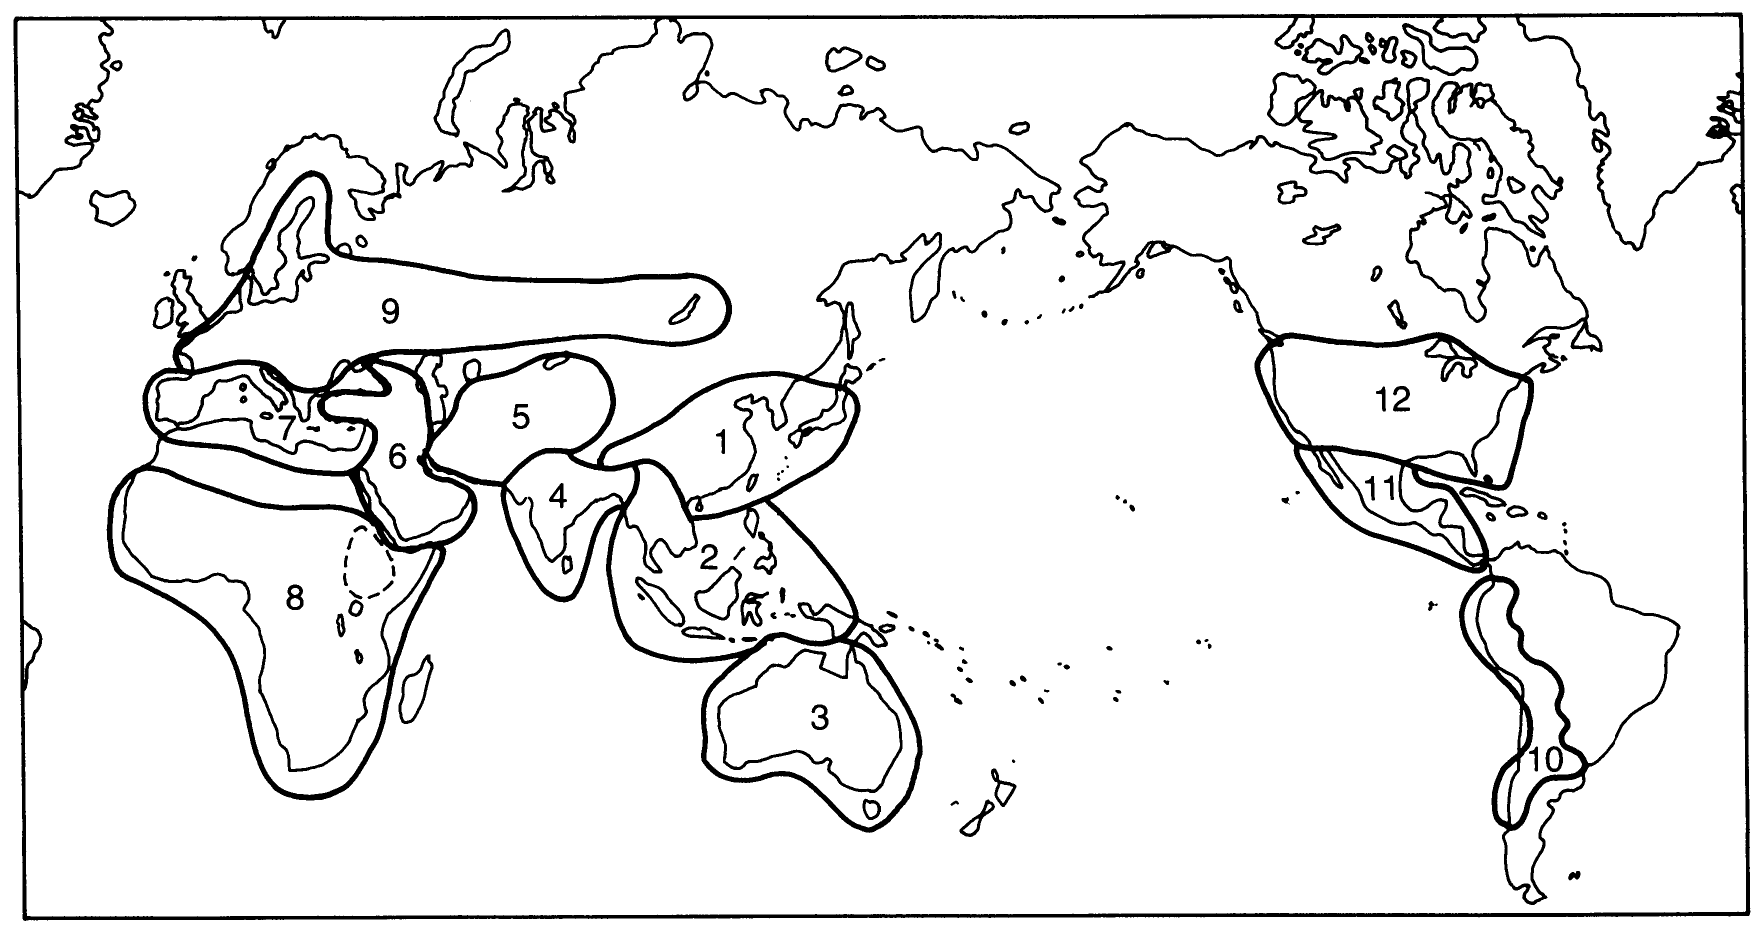
\includegraphics[width=0.55\linewidth]{./../images/megacentres_cultivated} \caption{Megacentres of cultivated plants (Zeven and Zhukovsky, 1975); @hayward2012plant, Page 37}\label{fig:cultivated-megacentres}
\end{figure}

\end{frame}

\begin{frame}{}
\protect\hypertarget{section-11}{}

\begin{table}[t]

\caption{\label{tab:diversity-region1}Cultivated plants and their regions of diversity. Based on Zeven and Zhukovsky (1975) and Zeven and de Wet (1982); @hayward2012plant, Page 54, 55.}
\centering
\fontsize{6}{8}\selectfont
\begin{tabular}{>{\raggedright\arraybackslash}p{3em}>{\raggedright\arraybackslash}p{14em}>{\raggedright\arraybackslash}p{32em}}
\toprule
SN & Region & Crops\\
\midrule
\rowcolor{gray!6}  1 & Chinese-Japanese region & Prosomillet, Foxtail millet, Naked oat\\
 &  & Soybean, Adzuki bean\\
\rowcolor{gray!6}   &  & Leafy mustard\\
 &  & Orange/Citrus, Peach, Apricot, Litchi\\
\rowcolor{gray!6}   &  & Bamboo, Ramie, Tung oil tree, Tea\\
\addlinespace
2 & Indochinese-Indonesian region & Rice\\
\rowcolor{gray!6}   &  & Rice bean, Winged bean\\
 &  & Cucurbits/Ash gourd\\
\rowcolor{gray!6}   &  & Mango, Banana, Rambutan, Durian, Bread fruit, Citrus/Lime, Grapefruit\\
 &  & Bamboos, Nutmeg, Clove, Sago-palm, Ginger, Taros and Yams, Betel nut, Coconut\\
\addlinespace
\rowcolor{gray!6}  3 & Australian region & Eucalyptus, Acacia, Macadamia nut\\
4 & Hindustani region & Rice, Little millet\\
\rowcolor{gray!6}   &  & Black gram, Green gram, Moth bean, Rice bean, Dolichos bean, Pigeonpea, Cowpea, Chickpea, Horsegram, Jute\\
 &  & Eggplant, Okra, Cucumber, Leafy mustard, Rat's tail radish, Taros and Yams\\
\rowcolor{gray!6}   &  & Citrus, Banana, Mango, Sunhemp, Tree cotton\\
\bottomrule
\end{tabular}
\end{table}

\end{frame}

\begin{frame}{}
\protect\hypertarget{section-12}{}

\begin{table}[t]

\caption{\label{tab:diversity-region2}Cultivated plants and their regions of diversity. Based on Zeven and Zhukovsky (1975) and Zeven and de Wet (1982); @hayward2012plant, Page 54, 55.}
\centering
\fontsize{6}{8}\selectfont
\begin{tabular}{>{\raggedright\arraybackslash}p{3em}>{\raggedright\arraybackslash}p{14em}>{\raggedright\arraybackslash}p{32em}}
\toprule
SN & Region & Crops\\
\midrule
\rowcolor{gray!6}   &  & Sesame, Ginger, Turmeric, Cardamom, Arecanut, Sugarcane, Black pepper, Indigo\\
5 & Central Asian region & Wheat (Bread/Club/Shot), Rye\\
\rowcolor{gray!6}   &  & Allium/Onion, Garlic, Spinach, Peas, Beetroot, Faba bean\\
 &  & Lentil, Chickpea\\
\rowcolor{gray!6}   &  & Apricot, Plum, Pear, Apple, Walnut, Almond, Pistachio, Melon, Grape, Carrot, Radish\\
\addlinespace
 &  & Hemp/Cannabis, Sesame, Flax, Safflower\\
\rowcolor{gray!6}  6 & Near Eastern region & Wheat (Einkorn, Durum, Poulard, Bread), Barley, Rye/Secale\\
 &  & Faba bean, Chickpea, French bean, Lentil, Pea\\
\rowcolor{gray!6}   &  & Brassica oleracea, Allium, Melon, Grape, Plum, Pear, Apple, Apricot, Pistachio, Fig, Pomegranate, Almond\\
 &  & Safflower, Sesame, Flax\\
\addlinespace
\rowcolor{gray!6}   &  & Lupins, Medics\\
7 & Mediterranean region & Wheat (Durum, Turgidum), Oats\\
\rowcolor{gray!6}   &  & Brassica oleracea, Lettuce, Beetroot, Colza\\
 &  & Faba bean, Radish\\
\rowcolor{gray!6}   &  & Olive, Trifolium/Berseem, Lupins, Crocus, Grape, Fennel, Cumin, Celery, Linseed\\
\bottomrule
\end{tabular}
\end{table}

\end{frame}

\begin{frame}{}
\protect\hypertarget{section-13}{}

\begin{table}[t]

\caption{\label{tab:diversity-region3}Cultivated plants and their regions of diversity. Based on Zeven and Zhukovsky (1975) and Zeven and de Wet (1982); @hayward2012plant, Page 54, 55.}
\centering
\fontsize{6}{8}\selectfont
\begin{tabular}{>{\raggedright\arraybackslash}p{3em}>{\raggedright\arraybackslash}p{14em}>{\raggedright\arraybackslash}p{32em}}
\toprule
SN & Region & Crops\\
\midrule
\rowcolor{gray!6}  8 & African region & Wheat (Durum, Emmer, Poulard, Bread)\\
 &  & African rice, Sorghum, Pearl millet, Finger millet, Teff\\
\rowcolor{gray!6}   &  & Cowpea, Bottle gourd, Okra, Yams, Cucumber\\
 &  & Castor bean, Sesame, Niger, Oil palm, Safflower, Flax\\
\rowcolor{gray!6}   &  & Cotton, Kenaf, Coffee\\
\addlinespace
 &  & Kola, Bambara, Groundnut, Date palm, Ensete, Melons\\
\rowcolor{gray!6}  9 & European-siberian region & Peach, Pear, Plum, Apricot, Apple, Almond, Walnut, Pistachio, Cherry\\
 &  & Cannabis, Mustard (black), Chicory, Hops, Lettuce\\
\rowcolor{gray!6}  10 & South American region & Potato, Sweet potato, Xanthosoma\\
 &  & Lima bean, Amaranth, Chenopodium, Cucurbita, Tomato, Tobacco, Lupin\\
\addlinespace
\rowcolor{gray!6}   &  & Papaya, Pineapple\\
 &  & Groundnut, Sea island cotton\\
\rowcolor{gray!6}   &  & Cassava, Cacao, Rubber tree, Passion fruit\\
11 & Central American and Mexican region & Maize, French bean, Potato, Cucurbita, Pepper/Chilli, Amaranth, Chenopodium, Tobacco, Sisal hemp, Upland cotton\\
\rowcolor{gray!6}  12 & North American region & Jeruselum artichoke, Sunflower, Plum, Raspberry, Strawberry\\
\bottomrule
\end{tabular}
\end{table}

\end{frame}

\hypertarget{plant-introduction}{%
\subsection{Plant introduction}\label{plant-introduction}}

\begin{frame}{Background}
\protect\hypertarget{background-1}{}

\begin{itemize}
\item
  The plant breeder may import new, unadapted genotypes from outside the
  production region, usually from another country (called plant
  introductions). These new materials may be evaluated and adapted to
  new production regions as new cultivars, or used as parents for
  crossing in breeding projects.
\item
  Primary Introduction

  \begin{itemize}
  \tightlist
  \item
    When the introduced variety is well adapted to the new environment,
    it is released for commercial cultivating without any alteration in
    the original genotype; this constitutes primary introduction. It is
    less common, particularly in countries having well organized crop
    improvement programmes.
  \end{itemize}
\item
  Secondary introduction

  \begin{itemize}
  \tightlist
  \item
    The introduced variety may be subject to selection in order to
    isolate a superior variety. Alternatively, it may be hybridized with
    local varieties to transfer one or few characters from these
    varieties to the local ones. Such introduction constitutes secondary
    introduction. It is much common than primary introduction.
  \end{itemize}
\end{itemize}

\end{frame}

\begin{frame}{Purpose}
\protect\hypertarget{purpose}{}

\begin{enumerate}
\tightlist
\item
  To obtain entirely new crop species
\item
  To serve as new varieties
\item
  For use in crop improvement programmes
\item
  To introgress variability to existing genetic materials
\item
  For scientific studies
\item
  To augment aesthetics
\item
  For germplasm collection and comparison
\end{enumerate}

\end{frame}

\hypertarget{bibliography}{%
\section*{Bibliography}\label{bibliography}}
\addcontentsline{toc}{section}{Bibliography}

\hypertarget{refs}{}
\leavevmode\hypertarget{ref-kingsbury2009hybrid}{}%
Kingsbury, Noel. 2009. \emph{Hybrid: The History and Science of Plant
Breeding}. University of Chicago Press.

\end{document}
